\documentclass[aspectratio=169]{beamer}

\usepackage[english]{babel}
\usepackage{graphicx}
\usepackage{media9}
\usepackage[absolute, overlay]{textpos}
\usepackage{multicol}
\usepackage{tikz}

\usetheme{Madrid}
\usecolortheme{crane}
\setbeamertemplate{page number in head/foot}{}
\setbeamertemplate{navigation symbols}{}

\title{Automatic Generation of Safety-Critical Test Scenarios\\for Collision Avoidance of Road Vehicles}
\author{Matthias Althoff and Sebastian Lutz}
\institute{University of Passau}
\date{\today}
\titlegraphic{
\includegraphics[height=.10\textheight]{media/logoUniPassau.jpg}}

\newcommand{\includeFSVideo}[1]{%
    \begin{textblock*}{5pt} (0pt, 0pt)
        \includemedia[
            height=\paperheight,
            width=\paperwidth,
            addresource=#1,
            activate=pageopen,
            flashvars={source=#1&autoPlay=true&loop=true}
        ]{}{VPlayer9.swf}
    \end{textblock*}
}

\begin{document}

\begin{frame}[plain]
    \noindent\makebox[\textwidth]{%
        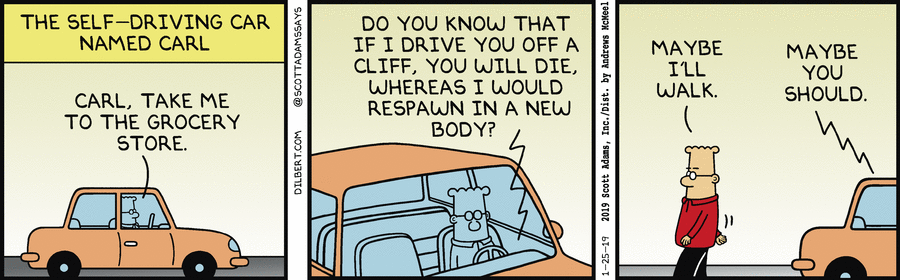
\includegraphics[width=.97\paperwidth]{media/2019-01-25_dilbert_autonomousCars.png}
    }
\end{frame}

\maketitle

\begin{frame}{Problems of other approaches}
\end{frame}

\begin{frame}{How this approach solves that}
\end{frame}

\begin{frame}{Measurement of criticality}
\end{frame}

\begin{frame}[plain] % Unoptimized scenario in driver view
    \includeFSVideo{./media/beamNG_driverView.mp4}
\end{frame}

\begin{frame}[plain] % Unoptimized scenario in free view
    \includeFSVideo{./media/beamNG_freeView.mp4}
\end{frame}

\begin{frame}[plain] % Development of drivable area
    \includeFSVideo{./media/drivableArea_development.mp4}
\end{frame}

\begin{frame}{Analyze development of drivable area}
    \begin{tikzpicture}
        \node[anchor=south west,inner sep=0] at (0,0) {\includegraphics[height=.95\textheight, trim=700 0 130 90, clip]{./media/drivableArea_development.png}};
        % \draw[red,thick,rounded corners]5 (3.7,5.7) rectangle (4.8,6.2);
        \onslide<2->{%
            \draw[red] (3.84,5.85) circle (1.6pt) node[anchor=west] {};
            \draw[red] (4.025,5.85) circle (1.6pt) node[anchor=west] {};
            \draw[red] (4.56,5.81) circle (1.6pt) node[anchor=west] {};
        }
    \end{tikzpicture}
\end{frame}

\end{document}
